\chapter{Kontextabgrenzung}

\section{Fachlicher Kontext}
\begin{figure}[H]
\begin{center}
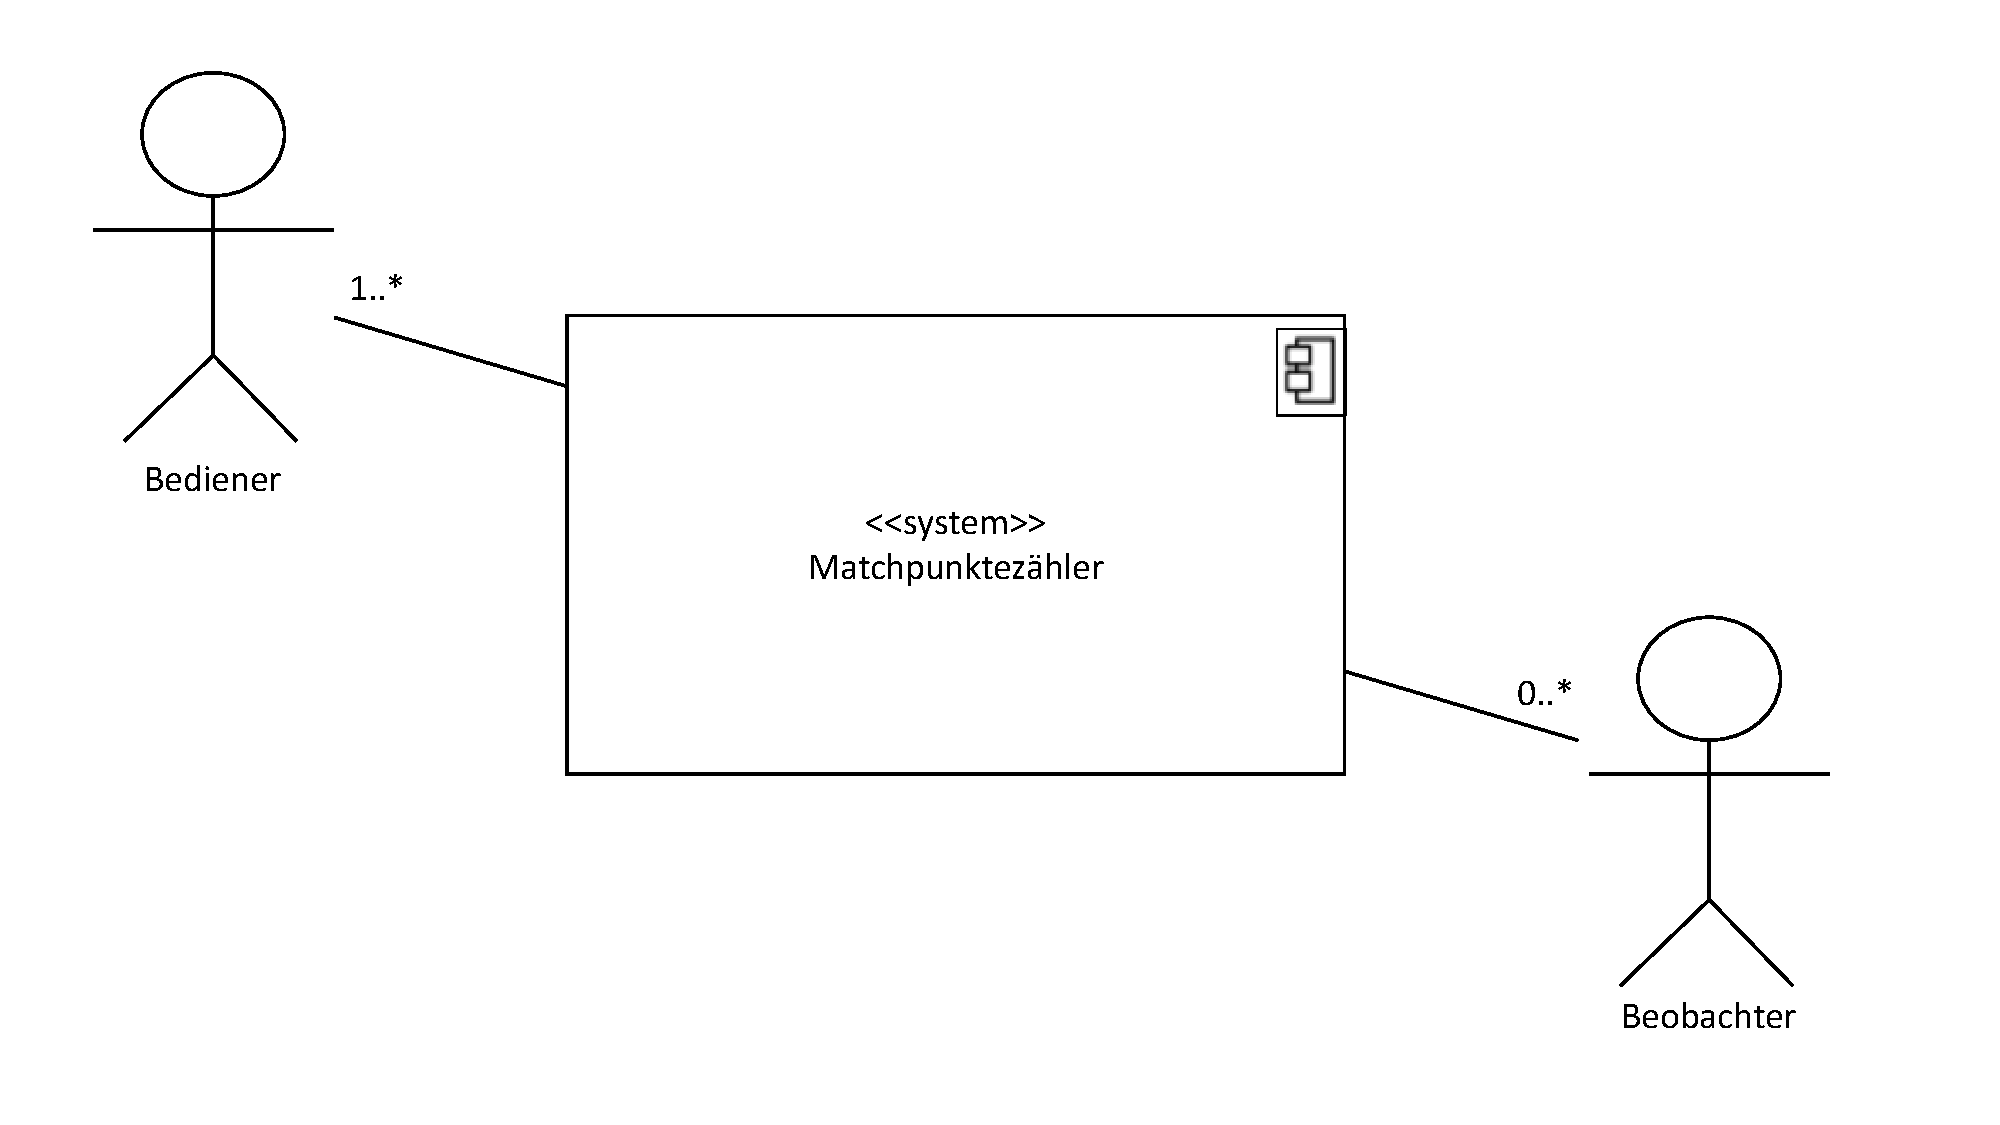
\includegraphics[scale=0.5]{Grafiken/FachlicherKontext.pdf}
\caption{FachlicherKontext}
\end{center}
\end{figure}

\subsection*{Bediener(Benutzer)}
Badminton wird mit mehreren Spieler gespielt. mindestens einer dieser Spieler muss zur Nutzung des Machtpunktezählers die Rolle des Bedieners übernehmen, um den Spielverlauf an das System zu übermitteln.
\subsection*{Beobachter(Benutzer)}
Jeder Mitspieler des Spiels ist an dem momentanen Spielstand interessiert und kann in die Rolle des Beobachters schlüpfen. Es besteht jedoch  die Möglichkeit, dass kein Spieler diese Rolle einnimmt, wenn der Spielverlauf lediglich dokumentiert werden soll.

\section{Technischer Kontext}
\begin{figure}[H]
\begin{center}
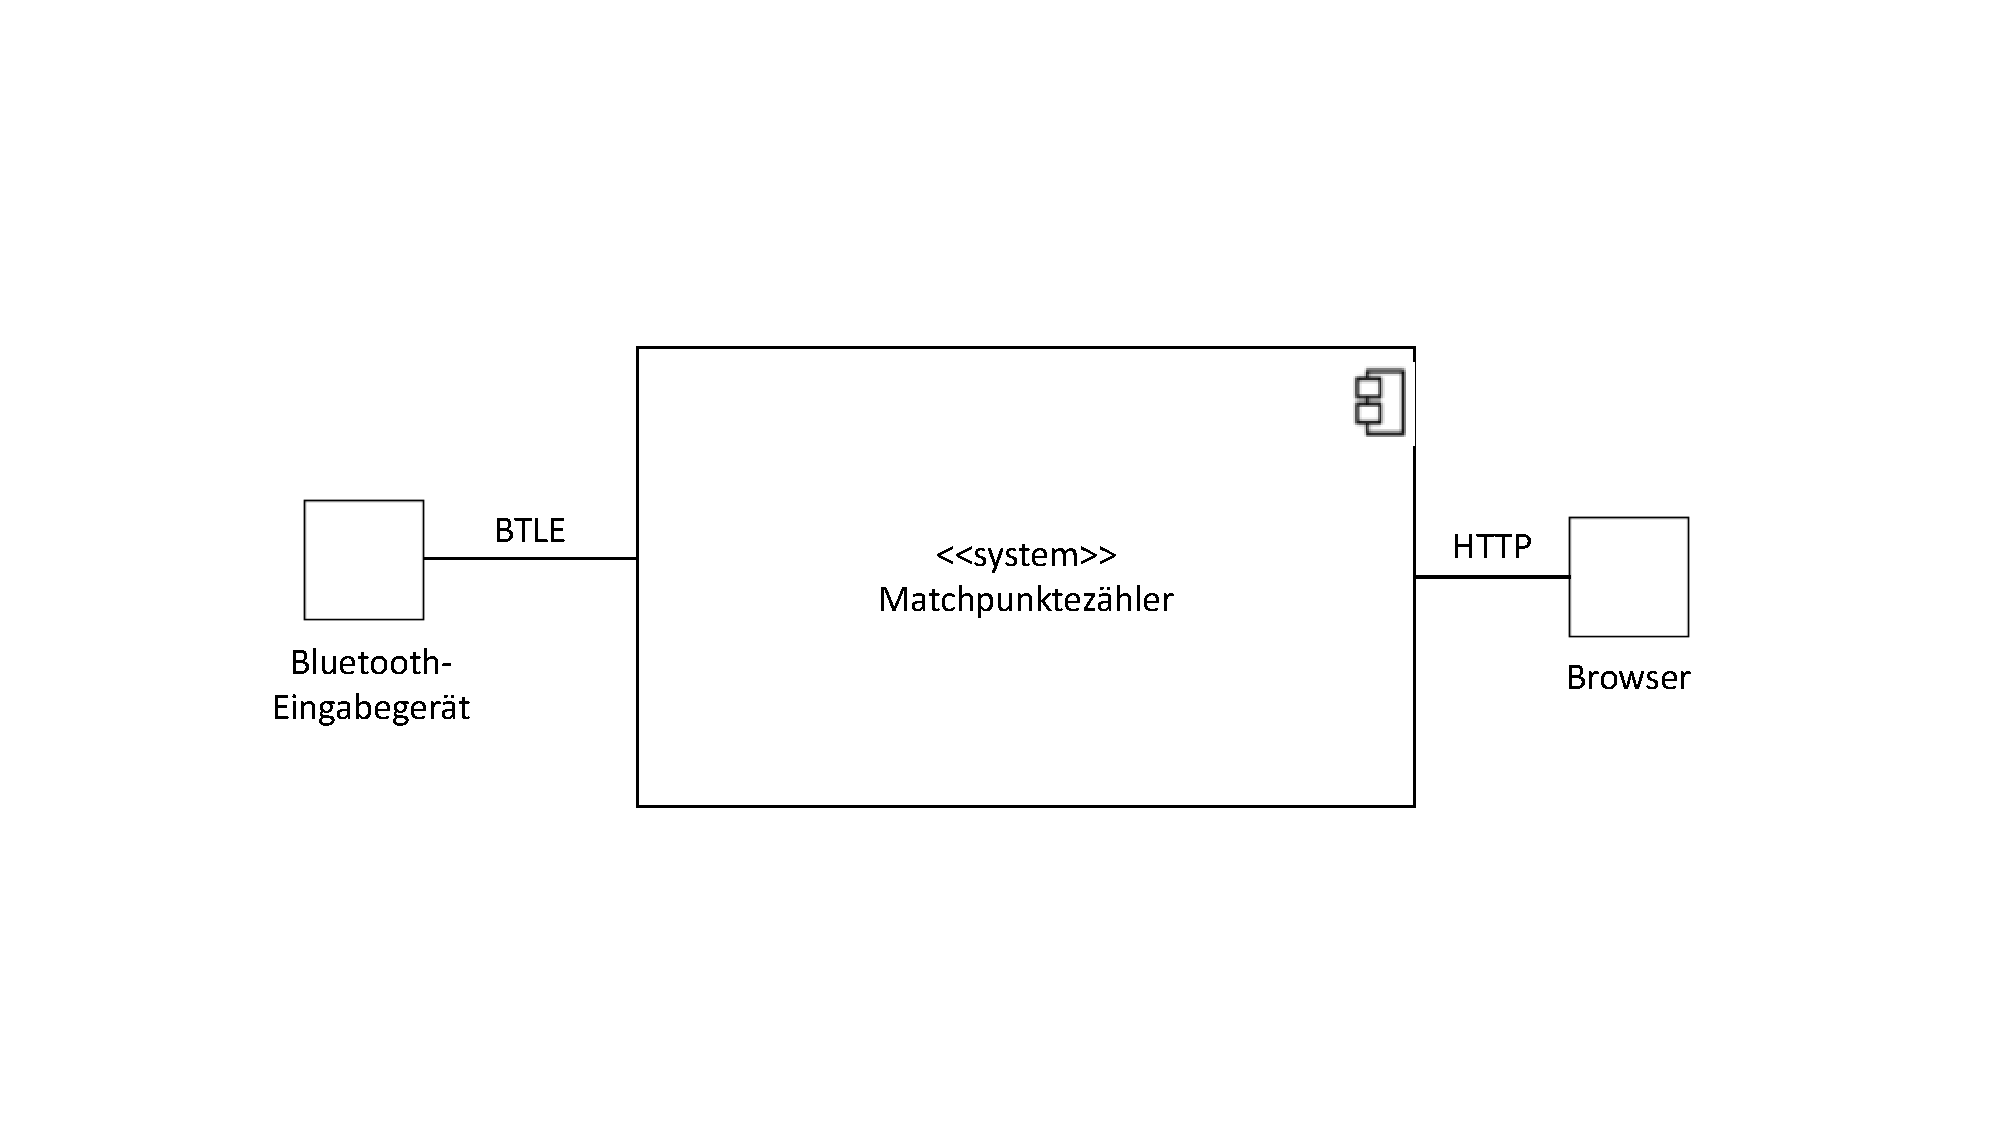
\includegraphics[scale=0.5]{Grafiken/TechnischerKontext.pdf}
\caption{TechnischerKontext}
\end{center}
\end{figure}

\subsection*{Bluetooth-Eingabegerät(Fremdsystem)}
Die Anbindung eines menschlichen Spielers als Bediener erfolgt durch ein Bluetooth-Eingabegerät. Dieses verbindet sich via Bluetooth-Low-Energy mit dem System und kann die Eingaben so entgegennehmen und übermitteln.
\subsection*{Browser(Fremdsystem)}
Der Browser bietet eine vielfältige Möglichkeit den aktuelle Stand des Systems auf unterschiedlichsten Endgeräten auszugeben. Dafür wird von einem Webserver über das HTTP-Protokoll eine Webseite für die Webbrowser bereitgestellt.
